% vim:textwidth=70:lines=42
\chapter{分布式数据分发的优化策略选择研究}
\label{chap:bt}

将分布式系统部署到一组数量巨大的节点上去是在系统运营准备阶段管理分布式
系统的任务之一。数据分发是分布式系统部署等应用的基础。临近邻居选择和动
态上传带宽分配是两种优化分布式数据分发的方法。本章在真实Internet测量数
据的基础上,对这两种优化方法进行了广泛而深入的研究测试,探索了应用这两
种优化方法的策略选择问题。得到了如下重要结论:临近邻居优化效果随临近邻
居比率增加而单调增加,其优化效果依赖于LRF块选择算法;使用贪心算法确定
的上传带宽分配策略使优化效果达到了局部最优,并且不依赖LRF块选择算法;
合并使用两种优化方法并不具有叠加优化效果。这些结论对实际系统应用具有重
要指导意义。

\section{本章引言}

%motivation: large file distribution in cooperative peers.
%problem: improve performance
% 说清楚一个应用场景,作为文章的backbone

数据分发技术是很多分布式应用的基础。P2P的文件共享系统将电影、歌曲和软
件CD等大文件分发给系统的每个用户。通过用户间合作下载,共享系统能够获得
几乎无限制的扩展性,同时,大大降低了数据源的负载。由文件共享系统产生的
数据传输,已经占了Internet流量的很大一部分。除此之外,人们还利用数据分
发技术,有效地将数据在CDN网络内部分发~\cite{fastreplica}。或者将这项技
术应用在分布式文件系统~\cite{sharkfs},让文件系统的用户安全地发现与下
载相互拥有的文件块,降低了服务器的压力。

数据分发的主要问题是将数据,尤其是大文件数据,分发到数量众多的用户或者
机器上。解决这个问题通常使用的基本技术是将文件分为逻辑上连续的若干块,
系统用户或者节点交换相互拥有的文件块,而不是直接向数据源服务器请求数据。
这样做的好处是显然的,首先降低了服务的压力,其次,这样的设计具有很好的
可扩展性,随着系统规模增大,总体的传输带宽也会增大。再次,文件块级别的
操作提供了更细粒度的负载均衡,从而系统节点能够动态的调整下载策略,绕开
可能的网络错误,以及获取更高下载性能。

进一步的,可以根据节点之间的通信拓扑将数据分发系统分为两种类型。swarm
类型的分发系统使用了随机连接拓扑,系统节点可以与任意其它节点通信。而
stream类型的系统使用了树、森林或者mesh等有约束结构的拓扑将节点连接起来。
swarm类型分发系统产生时间较stream类型系统更早。
BitTorrent~\cite{bittorrent}是swarm系统的代表。BitTorrent使用一个集中
式目录服务器记录系统节点与它们下载文件的进度。BitTorrent的客户端之间通
过这个目录服务器寻找可以提供文件块下载其他节点。目前,一些基于
BitTorrent协议的客户端也利用了DHT~\cite{kademlia}技术,实现了分布式结
构的目录服务器。基于stream方式的分发系统,包括
SplitStream~\cite{splitstream}和Bullet~\cite{bullet}等,试图通过使用精
巧的节点选择算法来解决负载均衡和传输效率问题,其结果是使系统节点构成了
树、森林或mesh等结构拓扑,并且在分发过程中使这一结构尽量稳定。这一方法
带来的好处是可能获得更高的聚集带宽,然而这需要节点之间的行为很好的同步,
因而对底层网络提出了更高的要求。在节点之间不能很好同步的情况下,stream
类型系统的传输效率会降低。

在Internet环境下基于swarm的分发技术得到了广泛应用。相比stream类型系统
,swarm更好的适应了Internet网络环境的动态变化,能够提供良好的传输性能
,同时也易于设计与实现。BitTorrent~\cite{bittorrent}文件共享协议是
swarm分发系统的典型代表。SharkFS~\cite{sharkfs}将swarm应用于分布式文件
系统,降低了文件服务器的负载。Coblitz~\cite{coblitz}将swarm应用于可控
的CDN网络,设计了基于HTTP协议的大文件分发下载服务。

% the point of paper
本文的研究内容始于一个基本的问题:如何提高swarm分发系统~\footnote{下文
中,分发系统都指基于swarm的分发系统}的性能?已有的工作从两方面指出了优
化的途径。\onlinecite{bns}通过模拟指出,使用临近邻居选择可以降低
BitTorrent的跨ISP流量,同时提高下载性能。然而~\onlinecite{bns}模拟使用
的网络拓扑过于简单,并不基于真实的网络数据。\onlinecite{taming,
zeroday}的工作使用了不同的技术,使临近邻居选择可以很容易的应用与部署到
实际分发系统。另一方面,\onlinecite{Bharambe2006}的工作显示了,固定上
传节点数目的带宽分配策略并不是最优的,动态的带宽分配策略可能会进一步提
高分发性能。

% 通过比较相关工作,引出本文的内容
% 说明两种优化方法都是已有的,但是没有详细的研究

虽然已有工作已经在提高分发系统性能方面做出了很多工作,然而还有很多问题
尚未仔细研究。本文通过在真实Internet测量数据上广泛的模拟测试,对这两种
优化方法的策略选择进行了仔细研究,得到了如下有实际指导意义的结论:

% contribution?

\begin{itemize}

  \item 临近邻居优化方法可以提高分发性能。随着临近节点占节点邻居列表的
  比例越来越高,系统的分发性能也单调提高,在邻居列表完全使用临近节点时
  达到最优。

  \item 动态上传带宽分配方法可以使用贪心算法确定上传节点的数目,提高了
  分发的聚集吞吐量,其优化效果达到了局部最优。
  
  \item 两种优化方法对数据块选择策略敏感程度不同。临近邻居选择优化依赖
  于LRF数据块选择算法,而上传带宽分配方法对数据块选择策略不敏感。

  \item 合并两种优化方法并不具有明显的叠加效果。实际应用中只需要选择一
  种优化方法应用。

\end{itemize}

本章接下来的内容安排如下。首先在\ref{sec:btmethod}节具体叙述两种优化方
法,并在\ref{sec:bteval}节对它们的应用策略选择进行广泛的实验性研究。在
\ref{sec:btsuggest}节讨论了在实际应用中应用优化方法需要考虑的问题,并
在\ref{sec:btconclude}节做小结。

%\section{或者:临近节点选择、带宽分配、文件块选择}

\section{优化方法概述}
\label{sec:btmethod}

本节首先给出分发系统的一般模型,接着叙述两种分发性能优化途径:临近邻居
选择和动态上传带宽分配。并在下一章研究应用这两种优化方法的策略。

\subsection{分发系统模型}

一般来说,一个数据分发系统可以用如下模型描述。

一个分发系统包括一个目录服务器和一组参与数据分发的节点。目录服务器维护
着节点列表与节点下载文件的进度。节点通过向目录服务器发送请求,获知系统
内其它节点的状态,包括节点列表与节点下载进度。同时,节点也会向目录服务
器更新自己的下载进度。分发系统的节点通过相互交换文件块完成文件下载,达
到数据分发的目的。

% 如何说的足够general,又能让基于bt的eval有说服力?

对一个分发系统来说,邻居选择、上传带宽分配和文件块选择是决定系统性能的
关键设计点。邻居选择是指节点向谁请求数据。分发系统中的节点数目众多,节
点可以从许多其它节点那里请求数据,尝试向每一个系统节点发送数据请求是效
率低下的,需要从中选择其中的一些作为自己的邻居,并从邻居节点获取数据块。
一个数据分发系统中,节点在获取数据的同时,还要满足来自其它节点的数据请
求。由于请求数目可能很大,如何分配上传带宽也是需要考虑的设计内容。节点
请求数据的单位是文件块,在同时有多个文件块需要下载的情况下,选择哪一块
下载是文件块选择需要决定的内容。

一个分发系统,无论其应用场景、具体设计方法如何不同,都可以从邻居选择、
上传带宽分配和文件块选择这三个方面描述其分发协议的设计。

BitTorrent使用了随机的邻居选择策略。中心目录服务器(tracker)返回一组
随机节点,BitTorrent的节点和邻居交换相互的数据块位图,得知对方已有的数
据块集合。BitTorrent通常使用LRF算法确定数据块的下载优先级,也就是会优
先下载所有邻居中副本最少的数据块。这样的方法能够很好的解决最后一块数据
块需要很长时间才能下载的问题。BitTorrent会优先给那些给自己上传过数据的
节点上传数据,并且对方上传带宽越大,优先级越高。采用这样的策略是因为
BitTorrent是为用户参与的P2P系统设计的,因而需要一定的激励机制,防止
free-rider的发生。已有的研究显示,BitTorrent的设计使得系统性能接近最优
解。

与BitTorrent不同,SharkFS使用了不同的邻居选择、上传带宽分配和文件块选
择策略。其本质是因为系统的应用场景不同。SharkFS实现了一个基于
DHT~\cite{coral}的分布式目录服务器。其邻居选择策略是选择最近的邻居,近
的定义是节点间延迟。SharkFS的节点对每一个需要下载的数据块,都会查询拥
有这个数据块的节点集合,并选择最近的节点请求数据。对于每个要下载的数据
块,SharkFS并不给出它们的下载顺序,因此是随机下载的。对于上传带宽分配
,SharkFS的文章中并未给出描述,我们可以认为是FIFO的。

% sharkfs: nearest peer, random piece, peer selection unspecified
% bittorrent: random peer, random/LRF, tit-for-tat
% 

% design figure

%节点选择和数据块选择的重要性。

本文考虑了两种提高分发性能的方法:选择临近节点作为邻居和动态上传带
宽分配。

\subsection{临近邻居选择}

%邻居选择,平均下载时间分析

临近邻居选择是指节点选择从“近”的邻居那里下载文件块。近的度量可以是节
点间延迟、带宽等网络连接属性,也可以是以延迟、带宽和丢包率为自变量的函
数值。从应用角度来看,以延迟时间(RTT)作为网络距离的度量是简单而有效
的方法。通常来看,延迟低的节点之间网络连接情况优于延迟高的节点。

% xxx: 分发树?and a bit of math

选择临近节点作为邻居列表从直观上来看是十分自然的。从单个节点来说,从近
处的节点下载文件块的速度更快,从而得到整个文件的时间更短。从整个分发系
统来说,完成整个文件分发的时间取决于每个文件块的分发时间,而每个文件块
的分发都动态构成一棵树。如果使用文件块传输时间为树上的边赋值,选择临近
节点后,分发树上的每条边的值以一定概率降低,从而整个分发性能得到提高。

换个角度说,一个分发系统实际上使用了epidemic算法分发数据,可以将这一过
程建模为一个分支过程,系统规模是$n$。如果只考虑一个数据块的分发过程,
每一轮每个节点都随机给其他$f$个节点传输一个数据块,在$r$轮之后,拥有这
个数据块的节点占整个系统的比例$Y_r$是:
\begin{equation}
\label{equ:epidemic}
Y_r \approx \frac{1}{1+ne^{-fr}} 
\end{equation}

分发固定比例$Y_r$需要的轮数$r$和$n$成$\log$关系,也就是$r =
O(\log(n))$。在实际系统中,完成每一轮都是需要时间的,因而分发固定比例
$Y_r$需要的时间可以近似表示为:
\begin{equation}
T = T_0 \times r
\end{equation}

$T_0$是传输一个数据块需要的平均时间。相对随机节点选择,临近邻居选择降
低了$T_0$的值,因而从根本上降低了系统的分发性能。

临近节点选择方法,可以有两种实现方式。第一种方式需要节点自己判断并选择
临近邻居。节点从目录服务器那里获知其它节点列表,而目录服务器并不了解节
点之间的网络连接特性,通常只会返回一组随机节点列表。得到这组列表后,节
点之间可以通过邻居列表的节点进行探测得到网络连接的特性。第二种方式是,
目录服务器直接返回一组临近节点,而节点并不知道返回的邻居节点的特性。这
样的设计只需要改变目录服务器,而不需要更改每个节点的设计,因而在实际中
更容易部署。

\subsection{动态上传带宽分配}

% 先给出intuition,然后分析,最后实现方式

分发系统中的一个节点可能会收到多个来自其它节点的请求,由于请求数量可能
是很多的,不可能同时满足请求的文件块。那么,按照什么顺序满足谁的请求就
是需要解决的问题。BitTorrent选择给固定数目的k(通常是5)个节点上传数据,
并且每10秒重新选择上传目标节点~\footnote{未包括乐观unchoke的情况}。这
样的静态带宽分配并不一定是性能最优的。\onlinecite{Bharambe2006}指出,
BitTorrent固定上传节点数目的分配方法并不是最优,动态调整上传节点数目可
以提高分发性能。

为了理解上传带宽分配的意义,我们举一个简单的例子。考虑一个三个节
点构成的分发系统,$v_1$, $v_2$, $v_3$。$v_1$的上传带宽是1,而$v_2$和
$v_3$上传带宽是2,它们的下载带宽无限制。初始时刻,$v_1$上有大小为1的数
据块。$v_1$可以将上传带宽平均分给$v_2$和$v_3$,从而在时刻2,$v_2$和
$v_3$都得到了数据块,整个系统完成了数据分发。另外一种上传带宽分配是
$v_1$将带宽全部分给$v_2$,在时刻1,$v_2$得到了整个数据块,同时给$v_3$
上传数据。在1.5时刻$v_3$也得到了数据块。从而整个系统在1.5时刻就完成了
数据分发。如果系统中包含其它节点,在时刻1,$v_1$就可以向其它节点传输数
据,分发的效率更加提高。

我们提出了基于贪心策略的上传带宽分配方法。数据分发系统的全局目标是在最
短时间内,让所有节点得到分发的文件。而分发的过程取决于每个节点的局部策
略。从这一角度来说,每个节点可以使用贪心策略通过局部最优使整个系统的性
能接近最优。具体地,每个节点应该使单位时间内上传的数据块数目最多。若设
节点的上传带宽是$u$,已有$m$个来自其它节点的数据块请求$q_1, q_2,
\cdots, q_m$,并且对应的可用传输带宽是$d_1, d_2, \cdots, d_m$,简单起
见,设$d_i > d_j, (i < j)$。为了尽快上传数据块,节点应该优先满足$q_1$
请求,如果上传带宽仍然有富余,再同时满足$q_2$请求。若设同时满足的请求
是$q_1$到$q_k$,则$k$应该满足如下条件:
\begin{equation}
\label{equ:bwalloc}
\left\{
\begin{array}{l}
\sum\limits_{i=1}^k d_i \ge u \\
\sum\limits_{i=1}^{k-1} d_i < u
\end{array}\right.
\end{equation}
% graph

%动态如何,静态如何,有什么问题。

从实现角度说,动态带宽分配实际上就是动态调整并发上传请求个数。而调整个
数的依据就是式子\ref{equ:bwalloc}的约束条件。这种优化方法需要让每个参
与分发系统的节点都调整自己的上传带宽分配策略,这是与临近邻居优化方法不
同的地方。从后面的评测可以看出,这样做虽然部署更困难一些,但是却带来来
了相对更优的优化性能。

\section{优化策略选择}
\label{sec:bteval}

我们已经叙述了临近邻居选择和动态上传带宽分配两种优化分发性能的方法。已
有工作确认了这两种方法可以优化分发性能。但是对优化策略的选择尚未仔细研
究。我们通过在真实Internet测量数据上的广泛模拟,通过实验性的方法,研究
了如下一些问题:1) 临近邻居选择通过在邻居集合中增加“近”处的节点,提
高数据块下载的效率,然而临近邻居比率在什么情况下会使分发性能最优?2)已
有工作\cite{Bharambe2006}显示了,BitTorrent的固定数目上传节点的策略并
不是最优,动态改变上传节点的个数,可以提高分发性能。本文指出,可以使用
贪心策略确定的约束条件(公式\ref{equ:bwalloc})确定上传节点集合。那么
这种策略是否是局部最优?3) 在分发系统设计中,不可避免的要考虑数据块选
择策略。已有两种被广泛使用的块选择策略:LRF (Least-Rarest-First)和随机
选择。LRF中,节点首先选择下载在所有邻居范围内,副本最少的数据块。这样
做是为了防止最后一个数据块很难下载的问题。随机数据块选择中,节点只是随
机请求自己没有的数据块。这两种数据块选择方法会影响临近邻居选择和动态上
传带宽分配的优化效果吗?4) 既然已知临近邻居选择和动态上传带宽分配可以
优化分发性能,那么自然的,合并这两种优化方法能否进一步改进分发性能呢?

下面,我们在基于模拟的广泛测试基础上,通过实际评测回答上面的问题,并给
出优化策略选择的结论与建议。

\subsection{评测方法}

我们使用基于BitTorrent的模拟器bitsim模拟200个节点的分发系统分发128MB文
件的行为。通过对比未优化和各种优化参数下的分发性能,研究不同优化策略的
效果。

模拟BitTorrent是因为BitTorrent是swarm类型分发系统的典型代表,它的行为
与性能得到了广泛的研究,其它swarm分发系统都采用了和BitTorrent相似的技
术。同时,BitTorrent的源代码也是公开的(版本5.0.9)之前,可以仔细分析
它的实现方式,实现尽可能相似的模拟结果。也可以在实际分布式计算平台上验
证模拟器是否和实际运行结果一致。而一些研究性系统或者商业系统由于无法实
际运行,因而难以设计实现相一致的模拟器。

bitsim模拟了标准的BitTorrent分发协议,包括choking/unchoking,乐观
unchoke,LRF块选择算法等。bitsim可以根据输入网络参数,模拟网络层的传输
延迟、TCP吞吐量和最大上传带宽。TCP的吞吐量依据流行的PFTK~\cite{pftk}模
型计算,模型中用到的窗口大小是$2^{16}$~Bytes。

模拟使用了200个节点的规模。为了得到具有代表性的真实Internet网络拓扑,
我们使用了iPlane~\cite{iplane}的数据。iPlane是一个网络测量服务,提供了
Internet上精确的网络间丢包率和延迟测量值。iPlane定期的参与到若干
BitTorrent分发系统中,以测量节点的上传带宽。模拟使用的200个节点是从
iPlane测量的节点集合中随机采样出的。在模拟中,200个节点在短时间内同时
进入分发系统。

% 节点加入退出

% metric
% 实验内容(bias,bwalloc,lrf...)

\subsection{临近邻居选择}

% 现象、趋势、小结论、原因、前提条件,讨论配置变化的影响
% 每个subsection后给出一个总结
% 直接看图和表就能说明问题

本小节探索临近邻居节点选择对分发性能的影响,回答了临近邻居比率多大时优
化效果最优。

在使用邻居邻居选择优化后,节点每次向tracker报告自己状态时,如果自身邻
居节点数量少于设定值,会向tracker请求返回系统内的若干其它节点(典型配
置是50)最为自己的邻居。我们希望选择临近的节点作为邻居会提高分发的性能,
因而tracker返回的节点包括两部分:临近节点和随机选择节点。但是这两部分
节点的数量、比率在什么情况下会是最优并不清楚。接下来我们通过实验测试的
办法给出结论。

首先需要验证临近邻居节点选择是否会提升数据分发性能。我们设定临近比率是
80\%。也就是是在tracker返回的节点列表中,80\%是以网络延迟为距离定义最
近的一组节点,剩下20\%是从系统中随机选择的若干节点。这样做的原因是避免
由于全部邻居节点都按照最近距离选择,造成网络分割的现象。

\begin{figure}[htbp]
  \centering
  \begin{minipage}{0.6\linewidth}
    \centering
    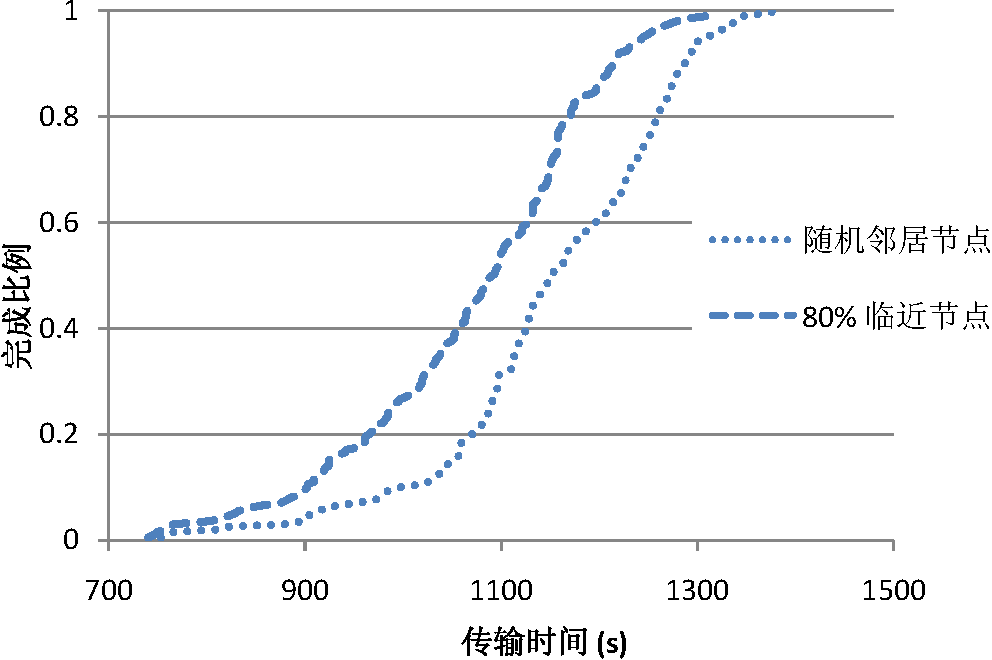
\includegraphics[width=1.0\linewidth]{bias80}
    \caption{临近邻居比率80\%时下载时间CDF曲线}
    \label{fig:bias80}
  \end{minipage}
\end{figure}

图~\ref{fig:bias80}是节点获取整个文件所用时间的累积分布函数(CDF),在
图中对比了使用随机邻居节点的结果和使用临近邻居节点选择的结果。从
整体上来看,采用临近邻居节点选择后,曲线相比正常实现向左有明显移动。这
意味着相同数量的节点完成下载所需的时间更少了。为方便对比,图~
\ref{fig:bias80}上的关键统计数据总结在表~\ref{tbl:bias80}中。

可以看出,相比随机邻居选择,80\%比率的临近邻居选择对下载性能有了一定改
进。下载时间中值从1150秒下降到了1093秒,性能改进是5.0\%;90\%的节点完
成下载时间从1288秒下降到了1214秒,性能改进是5.7\%;下载时间的平均值从
1151秒下降到了1071秒,性能改进是7.0\%。

\begin{table}[htbp]
\centering
\begin{minipage}{0.6\linewidth}
\centering
\caption{临近邻居比率80\%下载性能统计}
\label{tbl:bias80}
\begin{tabular}{lccc}

\toprule[1.5pt]
    & 中值 & 90\%完成 & 平均值\\
\midrule[1pt]
随机邻居选择  & 1150s & 1288s & 1151s\\
80\% 临近邻居 & 1093s & 1214s & 1071s\\
性能改进      & 5.0\% & 5.7\% & 7.0\%\\
\bottomrule[1.5pt]
\end{tabular}
\end{minipage}
\end{table}

这样的结果是符合我们的预期的。然而相对来说,优化效果并不一定是最优的。
为了找到更优的邻居选择策略,我们变化临近邻居选择的比率,并观察对下载性
能的影响。图~\ref{fig:biaschange}是临近邻居比率从20\%变化到100\%时,下
载时间的平均值和中值的变化情况。

\begin{figure}[htb]
  \centering
  \begin{minipage}{0.6\linewidth}
    \centering
    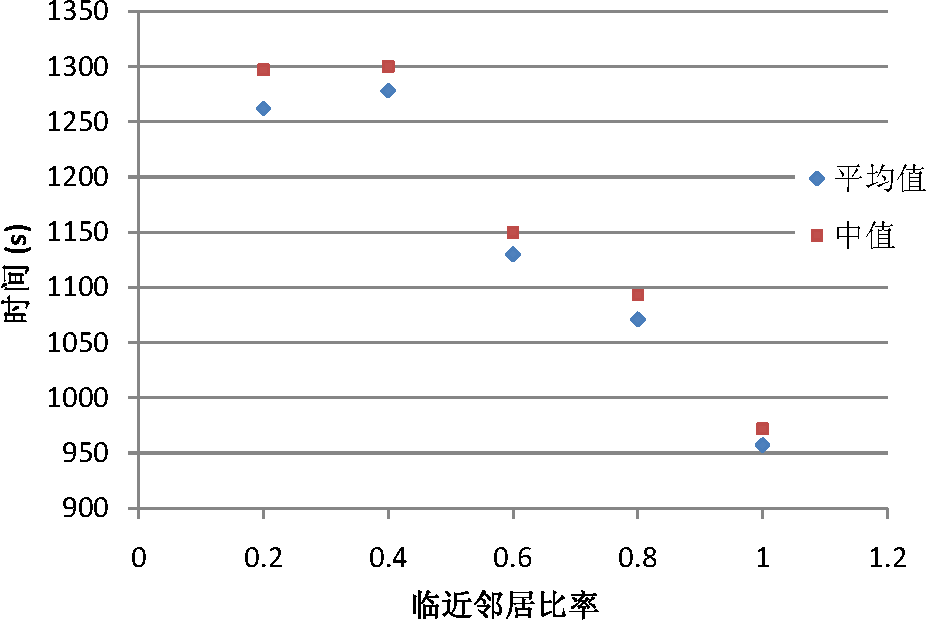
\includegraphics[width=1.0\linewidth]{biaschange}
    \caption{下载时间中值与平均值随临近邻居比率变化图}
    \label{fig:biaschange}
  \end{minipage}
\end{figure}

可以看出,随着节点选择更多的临近邻居,系统的整体性能呈现单调增长的趋势。
尤其需要注意的是,在100\%使用临近节点时,系统的性能达到了最优,其下载
时间CDF曲线如图~\ref{fig:bias10}所示。相比随机节点选择,分发进度的中值
从1150秒减少到了936秒,性能提高了18.6\%,90\%进度的时间从1288秒减少到
了1088秒,性能提高了15.5\%,分发时间的平均值1151秒减少到了916秒,性能
提高了20.4\%。

\begin{figure}[htb]
  \centering
  \begin{minipage}{0.6\linewidth}
    \centering
    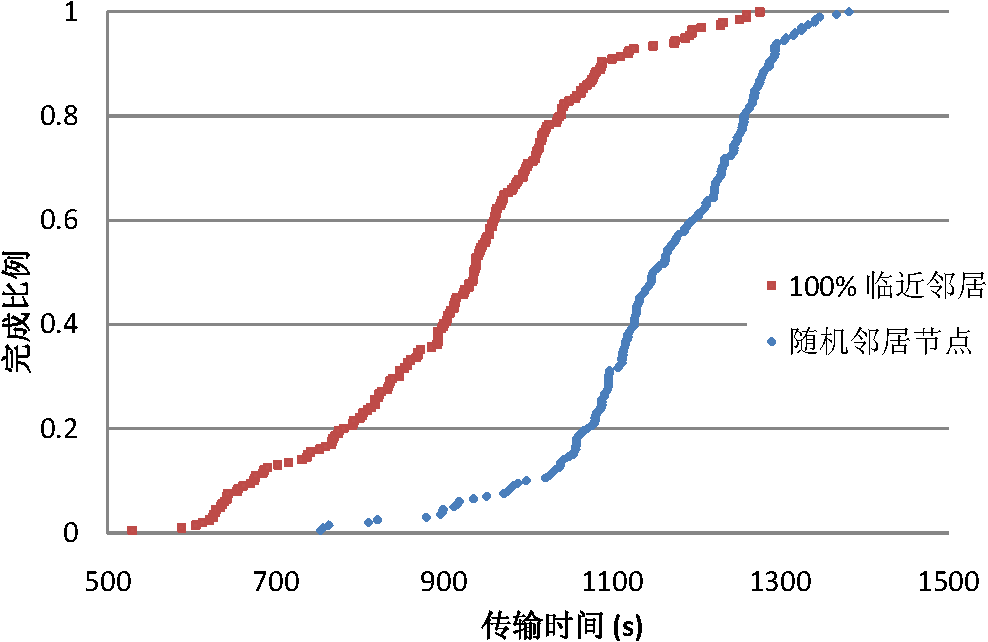
\includegraphics[width=1.0\linewidth]{bias10}
    \caption{临近邻居比率100\%时下载时间CDF曲线}
    \label{fig:bias10}
  \end{minipage}
\end{figure}

在使用100\%临近邻居时,没有发生担心的网络分割情况。这是因为节点的邻居
集合的度为50,其数量足够大,保证了很强的网络连通性。这样的结果告诉我们,
在实际分发系统设计中,可以使邻居节点包含尽可能多的临近节点,使分发性能
得到最大程度的提高。如果担心网络分割发生,只需要保留少数个随机选择的节
点就可以了。

\begin{table}[htbp]
\centering
\begin{minipage}{0.8\linewidth}
\centering
\caption{临近邻居比率100\%下载性能统计}
\label{tbl:bias10}
\begin{tabular}{lccc}

\toprule[1.5pt]
              & 中值 & 90\%完成 & 平均值\\
\midrule[1pt]
随机邻居选择  & 1150s & 1288s & 1151s\\
100\% 临近邻居 & 936 & 1088s & 916s\\
性能改进      & 18.6\% & 15.5\% & 20.4\%\\
\bottomrule[1.5pt]
\end{tabular}
\end{minipage}
\end{table}

%为了更仔细的研究系统特点,我们也收集了系统在分发文件过程中,节点的邻
%居分布

% 和系统总吞吐量的变化。

%图~\ref{fig:bias10path}
%
%\begin{figure}
%  \centering
%  \begin{minipage}{0.8\linewidth}
%    \centering
%    
\includegraphics[width=1.0\linewidth]{ph}
%    \caption{临近邻居延迟分布}
%    \label{fig:bias10path}
%  \end{minipage}
%\end{figure}

\textbf{结论}:通过测试我们发现,临近邻居选择可以提高分发系统的性能。
同时,随着临近节点占节点邻居列表的比例越来越高,系统的分发性能也单调提
高,在邻居列表完全使用临近节点时达到最优。

% path latency
% throughput

%1. 80\% bias: download time distribution, neighbour latency(需要重新测
%的), download rate from neighbours(可以从下载统计推导出)
%2. 不同bias
%3. 只保留若干长连接的bias

\subsection{上传带宽分配}

% xxx 模拟中,上传带宽分配优化是如何实现的

BitTorrent使用的固定上传节点数目的上传带宽分配策略并不是最优。我们给出
了基于贪心策略的动态上传带宽分配方法(式子~\ref{equ:bwalloc})。本小
节探索这种优化方法对分发性能的影响。

使用上传带宽分配优化后,相比未优化时,系统性能有了很大提高,节点下载文
件所用传输时间的累积分布函数如图~\ref{fig:bwalloc}所示。图中右边的曲线
是未优化时的传输时间分布,左边的曲线是使用上传带宽分配优化后的时间分布,
相比未优化的情况,有了明显的性能改进,直观的说,传输时间曲线向左有了明
显移动。

\begin{figure}[htbp]
  \centering
  \begin{minipage}{0.6\linewidth}
    \centering
    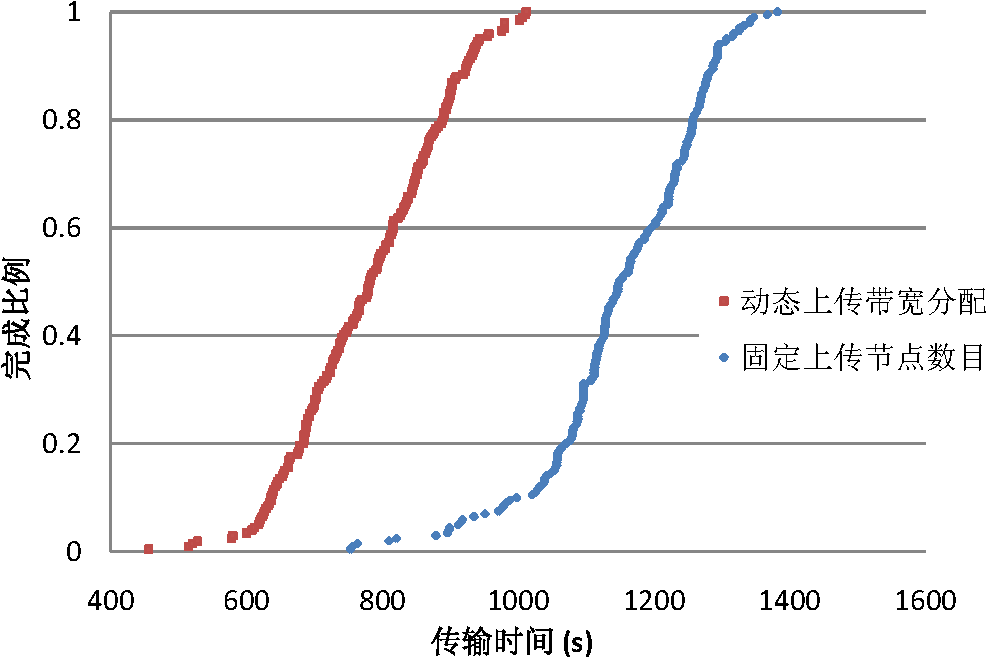
\includegraphics[width=1.0\linewidth]{bwalloc}
    \caption{上传带宽分配优化的下载时间CDF曲线}
    \label{fig:bwalloc}
  \end{minipage}
\end{figure}

从统计数据上看(表~\ref{tbl:bwalloc}),未优化时传输时间的中值是1150秒
,90\%完成时间是1288秒,传输时间的平均值是1151秒,而使用上传带宽优化后
,传输时间的中值减少到了782秒,性能提高了32.0\%,90\%完成传输时间减少
到了926秒,性能提高了28.1\%,传输时间的平均值减少到了780秒,性能提高了
32.2\%。

\begin{table}[htbp]
\centering
\begin{minipage}{0.8\linewidth}
\centering
\caption{上传带宽优化传输性能统计}
\label{tbl:bwalloc}
\begin{tabular}{lccc}

\toprule[1.5pt]
              & 中值 & 90\%完成 & 平均值\\
\midrule[1pt]
未优化    & 1150s & 1288s & 1151s\\
优化后    & 782   & 926s  & 780s\\
性能改进  & 32.0\% & 28.1\% & 32.2\%\\
\bottomrule[1.5pt]
\end{tabular}
\end{minipage}
\end{table}


%2. 提高了整体throughput, (bwalloc\_throughput)

上传带宽分配方法使得数据块尽可能快的从一个节点传输到另外一个节点,从整
体上看,提高了系统的聚集吞吐量。在试验中,我们统计了系统每20秒所有节点
新下载数据块的总量,计算出系统在这20秒内的平均聚集吞吐量。图~
\ref{fig:bwalloc_throughput}比较了使用和不适用上传带宽分配时,系统聚集
吞吐量的变化。从平均值看,优化前的平均吞吐量是17.47MB,优化后的平均吞
吐量是22.45MB,性能提高了28.5\%。

\begin{figure}[htb]
  \centering
  \begin{minipage}{0.6\linewidth}
    \centering
    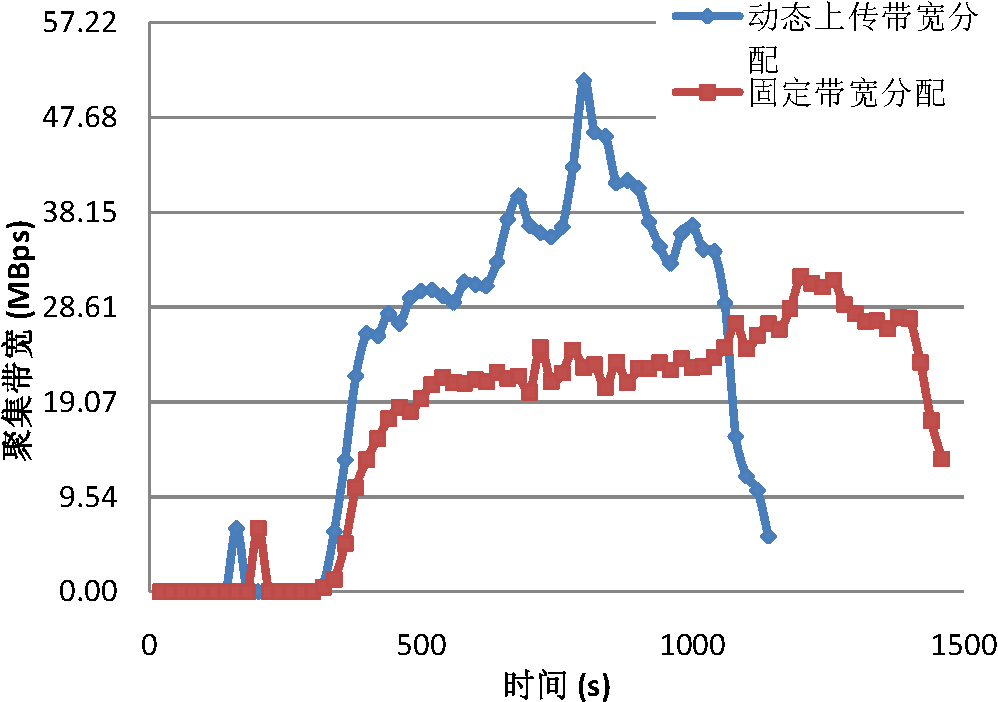
\includegraphics[width=1.0\linewidth]{bwalloc_throughput}
    \caption{动态上传带宽分配提高了聚集吞吐量}
    \label{fig:bwalloc_throughput}
  \end{minipage}
\end{figure}

%3. 与half,double对比 (bwalloc\_cmp)

动态带宽分配通过运行时动态调整上传节点个数来分配带宽,其优化效果达到了
局部最优。我们通过变化上传节点数目得到这一结论。假设动态带宽分配方法给
出的上传节点个数是$k$,我们将其与上传节点个数分别是$k/2$和$2k$的情况进
行对比。图~\ref{fig:bwalloc_cmp}是应用三种带宽分配方法得到的下载时间
CDF曲线。最左边的是标准分配方法的结果,右边的两个曲线是$k/2$和$2k$分配
方法的结果。可以看出,增大或者减小上传节点个数都会降低分发性能。$k/2$
的情况下,分发时间的中值和平均值分别是1024秒和1014秒,相比标准的情况性
能下降了30.9\%和30.0\%。$2k$的情况下,分发时间的中值和平均值分别是999
秒和995秒,相比标准的情况性能下降了27.7\%和27.6\%。

\begin{figure}[htb]
  \centering
  \begin{minipage}{0.6\linewidth}
    \centering
    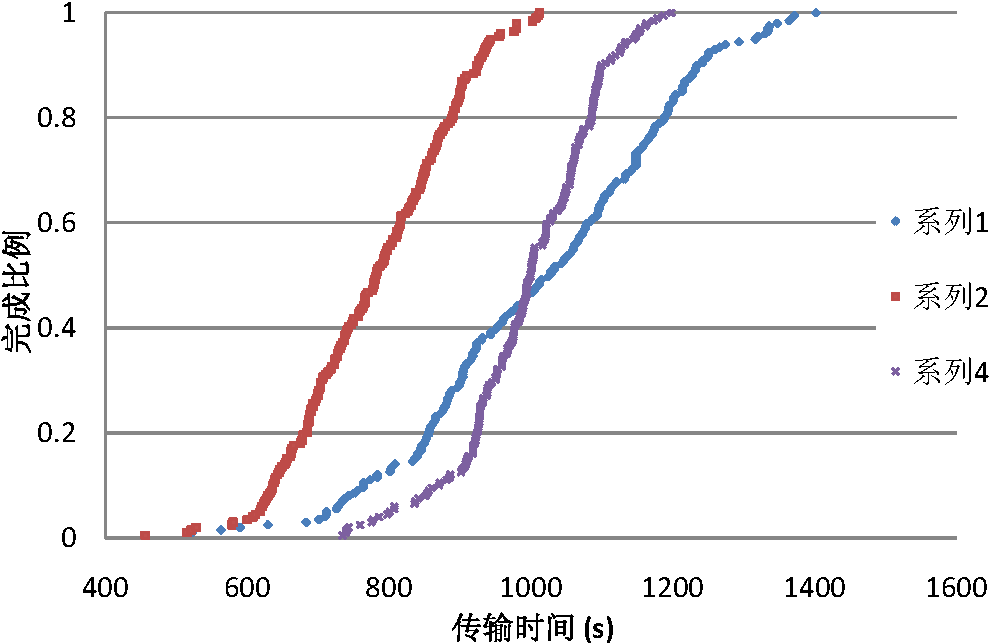
\includegraphics[width=1.0\linewidth]{bwalloc_cmp}
    \caption{不同上传带宽分配方法比较}
    \label{fig:bwalloc_cmp}
  \end{minipage}
\end{figure}

使用式子~\ref{equ:bwalloc}的上传带宽分配策略是局部最优的,这一结论是合
理的。使用式~\ref{equ:bwalloc},一个节点在自己上传带宽允许范围内,使数
据块请求被最快被满足,单位时间上传数据块的数目最多,从整体上提高了聚集
吞吐量。相对式~\ref{equ:bwalloc}确定的上传节点个数,如果减少上传节点数
目,则自身的上传带宽有部分未被使用,降低了上传效率,如果增加上传节点数
目,则上传数据块的时间增长,单位时间上传数据块的数目减少,也降低了上传
效率。

\textbf{结论}:动态上传带宽分配使用贪心策略在运行时动态调整上传节点数
据,提高了分发系统的聚集吞吐量,其优化效果达到了局部最优。

%4. 上传节点数量分布 (bwalloc\_upnode)
%图~\ref{fig:bwalloc_upnode}
%
%\begin{figure}
%  \centering
%  \begin{minipage}{0.8\linewidth}
%    \centering
%    
\includegraphics[width=1.0\linewidth]{ph}
%    \caption{}
%    \label{fig:bwalloc_upnode}
%  \end{minipage}
%\end{figure}

%5. 原因:因为这个方法会选择上传的节点,和bias用latency选择类似。只不过
%tracker没有帮助选择节点。比bias更好是因为分发truck的速度更快,考虑了自
%身上传带宽的因素。

\subsection{数据块选择策略的影响}

两种常见的数据块选择策略是随机选择和最少副本优先(LRF,
Least-Rarest-First)。在这里我们评测不同的数据块选择策略与两种优化方法
的相互影响。

\begin{figure}[htbp]
  \centering
  \begin{minipage}{0.6\linewidth}
    \centering
    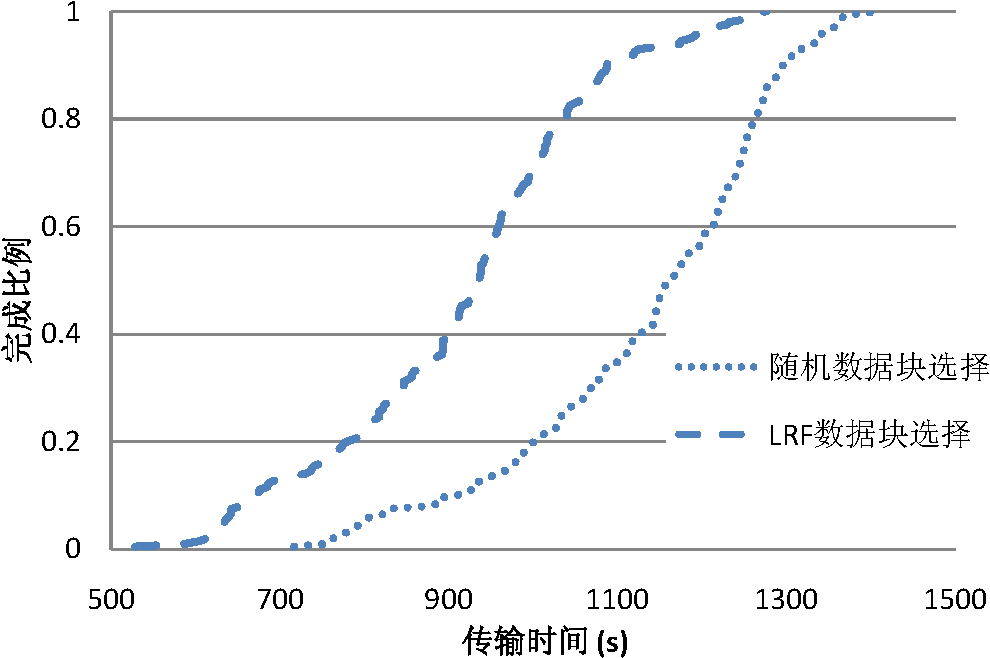
\includegraphics[width=1.0\linewidth]{bias_lrfvsrand}
    \caption{数据块选择对临近邻居优化的影响}
    \label{fig:bias_lrfvsrand}
  \end{minipage}
\end{figure}

首先我们比较使用不同的数据块选择策略是否对优化效果有影响。图~
\ref{fig:bias_lrfvsrand}和图~\ref{fig:bwalloc_lrfvsrand}分别显示了使用
随机和LRF数据块选择策略后,临近邻居选择和动态带宽分配的性能变化情况。
总体来说,随机数据块选择相比LRF都会降低系统性能,从图上看随机数据块选
择的曲线相比LRF的曲线向右移动。但是对两种优化的影响程度不同。使用随机
数据块选择后,临近邻居选择的性能下降更多一些。分发时间的中值从936秒增
加到了1161秒,性能下降了24.0\%,平均值从916秒增加到了1135秒,性能下降
了23.9\%。而动态上传带宽分配相对性能变化较小。分发时间的中值从782秒增
加到了828秒,性能下降了5.9\%,平均值从780秒增加到了822秒,性能下降了
5.4\%,可以说基本没有影响。

\begin{figure}[htb]
  \centering
  \begin{minipage}{0.6\linewidth}
    \centering
    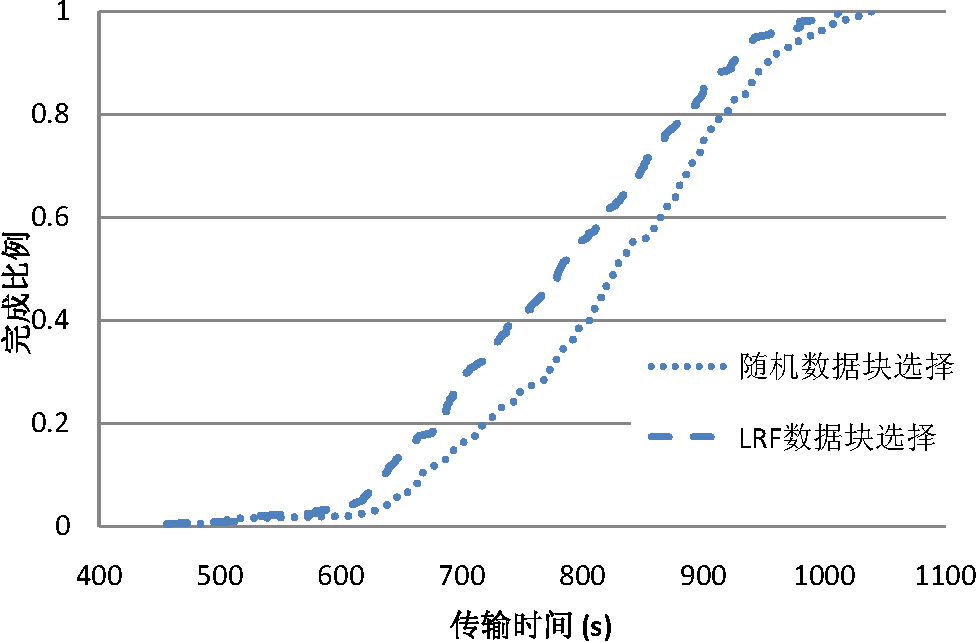
\includegraphics[width=1.0\linewidth]{bwalloc_lrfvsrand}
    \caption{数据块选择对动态上传带宽分配优化的影响}
    \label{fig:bwalloc_lrfvsrand}
  \end{minipage}
\end{figure}

之所以数据块选择对性能有影响,是因为不同的数据块选择策略会改变分发时数
据块在整个系统的分布情况。而两种优化方法对数据块的分布敏感程度不同,因
此造成性能有不同程度的变化。图~\ref{fig:diversity_bias}是使用临近邻居
节点优化时,在不同的数据块选择策略下数据块分布,上传带宽分配得到的结果
与图~\ref{fig:diversity_bias}类似。我们统计了在整体分发进度为30\%时,
数据块在系统内的分布情况。横轴是数据块的编号,纵轴是相同数据块在系统内
的副本数量。可以看出,在随机数据块选择时,数据块在系统内分布的不够均匀。
而使用LRF选择策略的情况则不同,基本上所有的数据块的副本数量都分布在一
个小的范围之内。

\begin{figure}[htb]
  \centering
  \begin{minipage}{0.6\linewidth}
    \centering
    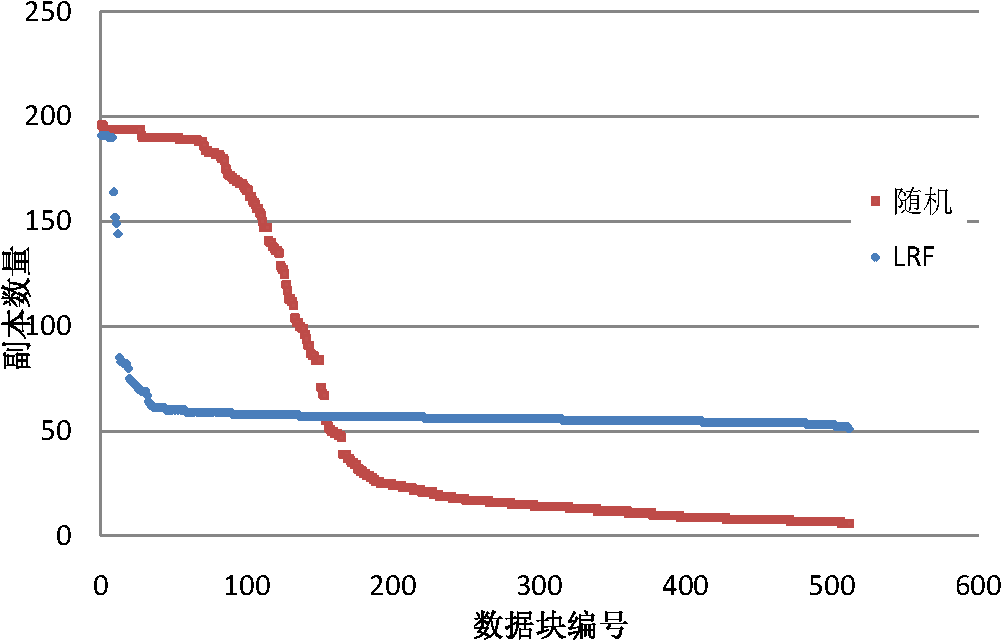
\includegraphics[width=1.0\linewidth]{diversity_bias}
    \caption{数据块副本分布}
    \label{fig:diversity_bias}
  \end{minipage}
\end{figure}

%图~\ref{fig:diversity_bwalloc}
%\begin{figure}
%  \centering
%  \begin{minipage}{0.8\linewidth}
%    \centering
%    
\includegraphics[width=1.0\linewidth]{ph}
%    \caption{}
%    \label{fig:diversity_bwalloc}
%  \end{minipage}
%\end{figure}

这就造成了对不同优化方法的影响程度不同。在临近邻居选择中,节点之间会有
聚类效应,也就是距离近的节点会成为相互的邻居。随机数据块选择让数据块的
分布不均匀,因而节点从邻居那里得到数据块的难度增大。采用LRF数据块选择,
数据块分布更加均匀,相近节点可以高效的交换相互没有的数据块。而上传带宽
优化并没有使用用随机邻居选择,因此没有邻居的聚类效应,LRF对分发性能的
影响也不大。

%3. 原因: a) lrf会增进性能 b)对带宽分配优化影响相对小: bias以后,相近的
%节点会有聚类效应,lrf能够很快的把类外的新的trunk拉回来。如果用random,
%则很可能得到的trunk是类内的,分发数据的效率受影响。

\textbf{结论}:两种优化方法对数据块选择策略敏感程度不同。临近邻居选择
优化依赖于LRF数据块选择算法,而上传带宽优化方法对数据块选择策略不敏感。
因而使用临近邻居优化方法必须配合使用LRF块选择算法。


\subsection{合并两种优化方法}

临近邻居选择和动态上传带宽优化都可以很好的提高分发性能,我们想要问,如
果同时应用这两种优化方法,是否会更进一步的优化系统性能呢?图~
\ref{fig:biasandbwalloc}回答了这个问题。可以看出合并后,性能有所提升,
但是不如单独应用一种优化方法带来的性能提升那样大。这是因为,采用临近邻
居后,邻居节点之间比较近,相互的传输带宽也比较好,因而再使用带宽分配优
化效果并不明显。

\begin{figure}[htbp]
  \centering
  \begin{minipage}{0.6\linewidth}
    \centering
    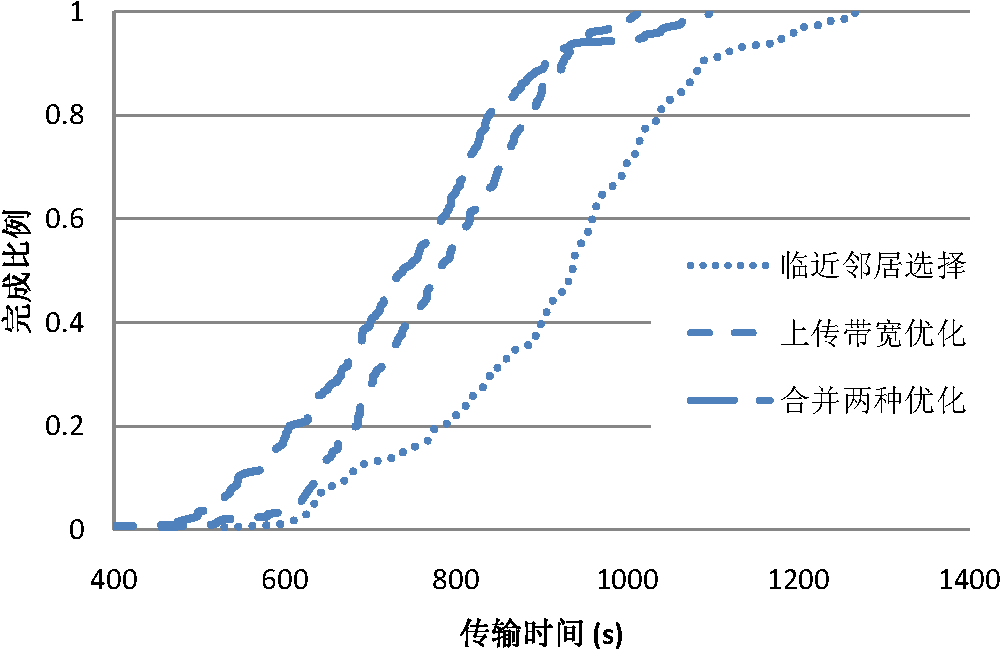
\includegraphics[width=1.0\linewidth]{biasandbwalloc}
    \caption{合并两种优化方法后传输时间分布}
    \label{fig:biasandbwalloc}
  \end{minipage}
\end{figure}

\textbf{结论}:合并两种优化方法并不具有明显的叠加效果。实际应用中只需
要选择一种优化方法应用。


%2. 不具有叠加效果: xxx: bias以后,节点就已经比较近了,相互之间传输带宽
%比较好,再使用带宽优化改进不大。

\section{实际应用策略讨论}
\label{sec:btsuggest}

我们对两种优化方法在实际系统中的应用策略进行讨论。

首先临近邻居选择和动态上传带宽分配都可以优化系统的性能,并且动态上传带
宽分配的优化效果稍好一些。应用临近邻居优化方法时临近,邻居比率越大优化
效果越好。动态上传带宽分配优化可以使用贪心策略确定上传节点数目,优化效
果达到局部最优。两种优化方法叠加使用并没有性能优化的叠加效果,因此实际
中只需选择其中一种应用。

两种优化方法在实际应用中都有不同的约束条件。临近邻居优化较为容易实现,
因为现有的技术可以保证只改变目录服务器的实现就可以应用此优化方法,但是
这种优化方法依赖于LRF数据块选择。上传带宽分配并不依赖特定的数据块选择
方法,然而应用这种优化方法需要改变每个节点的实现,因此部署起来比较麻烦。
对于由用户参与的P2P系统,可以使用临近邻居优化方法改进性能,对于处在单
个管理域的分布式系统,可以使用动态上传带宽分配方法获得比临近邻居选择方
法更优的分发性能。

\section{本章小结}
\label{sec:btconclude}

本章对分布式数据分发的优化策略选择进行了广泛研究。我们考虑了两种优化方
法,临近邻居选择和动态上传带宽分配。通过广泛而深入的实验研究,我们对它
们的优化效果、优化参数选择与依赖因素有了深入的认识,并对实际应用中的应
用策略进行了讨论。
